% main.tex -- The Efficiency Trap
% CS-GY 6033G Design and Analysis of Algorithms I, New York University
% Student ID N18349850
% Single-file; compiles with pdfLaTeX on Overleaf (TeX Live 2023+).

\documentclass[11pt]{article}

\usepackage[a4paper,margin=2.4cm,headheight=14pt]{geometry}
\usepackage[T1]{fontenc}
\usepackage[utf8]{inputenc}
\usepackage{lmodern}
\usepackage{microtype}
\usepackage{amsmath,amssymb,amsthm}
\usepackage{booktabs,array,tabularx}
\usepackage{xcolor}
\usepackage{fancyhdr}
\usepackage{algorithm}
\usepackage{algpseudocode}
\usepackage{enumitem}
\usepackage{tikz}
\usetikzlibrary{positioning,arrows.meta}
\usepackage[numbers,sort&compress]{natbib}
\usepackage[hidelinks]{hyperref}

\definecolor{ink}{HTML}{17171B}
\definecolor{accent}{HTML}{C2410C}

\newtheorem{proposition}{Proposition}
\newtheorem{lemma}{Lemma}
\theoremstyle{definition}
\newtheorem{definition}{Definition}
\theoremstyle{remark}
\newtheorem*{remark}{Remark}

\newcommand{\Wh}{\,\mathrm{Wh}}
\newcommand{\TWh}{\,\mathrm{TWh}}

\pagestyle{fancy}
\fancyhf{}
\fancyhead[L]{\small CS-GY 6033G \textperiodcentered{} New York University}
\fancyhead[R]{\small Student ID N18349850}
\fancyfoot[C]{\small\thepage}
\renewcommand{\headrulewidth}{0.4pt}
\hypersetup{pdftitle={The Efficiency Trap}, pdfauthor={NYU Student N18349850}}

\setlength{\parskip}{3pt}

\begin{document}

\begin{center}
  {\small\color{accent}\textsc{CS-GY 6033G: Design and Analysis of Algorithms I \quad\textperiodcentered\quad New York University}}\\[10pt]
  {\LARGE\bfseries\color{ink} The Efficiency Trap}\\[4pt]
  {\large Why Rapid Gains in AI Energy Efficiency Have Not Reduced AI's Electricity Demand,\\ and Which Algorithmic Interventions Can Make Them Count}\\[10pt]
  Student ID: N18349850 \qquad Submitted: November 2026
\end{center}

\begin{abstract}
\noindent
Turing showed in 1936 that one machine can compute anything computable; what he could not make free was the time it takes, and on real hardware time is electricity. The energy needed to answer a single generative-AI request is now falling faster than almost any efficiency trend in the history of energy: the International Energy Agency (IEA) reports reductions of at least an order of magnitude per year, and Google measured a $33\times$ reduction for its median Gemini text prompt in twelve months. Yet global data-centre electricity rose $17\%$ in 2025, and electricity for AI-focused data centres rose $50\%$. This paper asks why per-task efficiency has not reduced total demand, and what algorithms can and cannot do about it. We synthesise evidence from primary sources, separating production measurements, laboratory measurements, third-party estimates and projections, and use a multiplicative identity, $E=\sum_k N_k\,w_k\,\varepsilon$ and $C=\sum_t E_t\,c_t$, to show that the 2025 data imply task-weighted demand grew by roughly $15\times$, enough to absorb the efficiency gains (a rebound, or Jevons, effect): the solution became the problem. We analyse four interventions as algorithms (model routing, speculative decoding as a geometric series, batching as amortisation, and carbon-aware scheduling, for which we prove a greedy schedule optimal and give an $O(n)$ algorithm), and add a fifth that targets the total rather than each job: an energy budget spent by a multiple-choice knapsack. In a one-year simulation at IEA-implied growth rates, the budget holds energy flat; with the \emph{same} energy, a first-come-first-served rate limit (the mechanism AI providers already use) answers $61\%$ of requests, while the knapsack answers $100\%$, $95\%$ at full quality. Everything is implemented in \texttt{effitrap}, an open-source, model-agnostic tool that a developer adds with one line before each AI call; it is verified by 49 checks over 906 random cases, including a real recorded grid forecast and forecasts with deliberate $\pm30\%$ errors. Consistent with the No Free Lunch theorem, no intervention is free and none defeats the rebound alone: an algorithm can spend a budget well, but people must choose it.
\end{abstract}

\noindent\textbf{Keywords:} sustainable computing; large language models; inference efficiency; rebound effect; Jevons paradox; carbon-aware scheduling; knapsack; amortised analysis; greedy algorithms.
% =====================================================================
\section{Introduction}\label{sec:intro}

In 1936 Alan Turing described a single machine that can carry out any computation that can be carried out at all \citep{turing1936}. Modern AI is that machine at enormous scale, and the one thing the theory never made free is time: every step a computer takes draws power. Generative AI feels weightless to its users, but every answer is computed in a data centre that draws electricity from a grid. The physical scale is now large: a typical AI-focused data centre consumes as much electricity as $100{,}000$ households, and the largest under construction will consume twenty times as much \citep{iea2025}. Data centres worldwide used about $485\TWh$ in 2025, comparable to Germany's annual electricity generation and around $1.5\%$ of global electricity, and the IEA expects this to roughly double to about $950\TWh$ by 2030 \citep{iea2026,owid2026}.

At the same time, the energy cost of an individual AI task is collapsing. The IEA's 2026 update reports that software and hardware advances have cut energy per AI task by at least an order of magnitude per year, a pace it describes as unprecedented in energy history \citep{iea2026}. Google's production measurements show the median Gemini Apps text prompt using $0.24\Wh$ in May 2025, $33\times$ less energy than twelve months earlier \citep{elsworth2025}.

These two facts sit uneasily together. If each task is ten times cheaper every year, why is total consumption rising faster than ever? Our answer, in one line, is that \emph{the solution became the problem}: cheaper answers led to many more answers. Algorithms have a name for the broader lesson. The No Free Lunch theorem shows that, averaged over all problems, no optimisation algorithm beats any other \citep{wolpert1997}; every gain is paid for somewhere. We therefore report a ``price'' for every intervention we study. This paper addresses three research questions:
\begin{enumerate}[label=\textbf{RQ\arabic*.},leftmargin=*,itemsep=1pt]
  \item Why have large per-task efficiency gains not reduced aggregate AI electricity demand?
  \item Which technical interventions reduce energy or emissions, by how much, and through which mechanism?
  \item What conditions determine whether those reductions persist at the level of the whole system?
\end{enumerate}

\paragraph{Contributions.} (i) A factor identity that maps each intervention to the quantity it changes and makes the rebound effect explicit (\S\ref{sec:identity}); (ii) a quantitative reading of the 2025 data showing that demand growth absorbed the efficiency gains (\S\ref{sec:trap}); (iii) an evidence-graded taxonomy of interventions organised as four moves (\S\ref{sec:moves}); (iv) algorithmic analyses of batching, speculative decoding, budgeted model routing and carbon-aware scheduling, including an optimality proof and a linear-time algorithm for the last (\S\ref{sec:algorithms}); (v) a budget policy that caps total energy, compared in simulation against both per-job efficiency and the rate limits AI providers already use (\S\ref{sec:cap}); (vi) an open-source, model-agnostic implementation, \texttt{effitrap}, used through one line before each AI call, with an oracle-checked test suite, forecast-robustness tests and benchmarks (\S\ref{sec:impl}); and (vii) policy recommendations that follow from the analysis (\S\ref{sec:policy}).

% =====================================================================
\section{Method and Sources}\label{sec:method}

This is a structured synthesis rather than a new measurement study. The two anchor sources are the IEA's \emph{Energy and AI} report \citep{iea2025} and MIT Technology Review's investigation \citep{mittr2025}. We added the IEA's 2026 update \citep{iea2026}; Google's production measurement study \citep{elsworth2025}; peer-reviewed work on inference energy \citep{luccioni2024power}, training energy \citep{patterson2022}, cloud carbon intensity \citep{dodge2022}, carbon-aware scheduling \citep{radovanovic2023}, serving systems \citep{kwon2023}, speculative decoding \citep{leviathan2023}, quantisation \citep{dettmers2022} and rebound effects \citep{luccioni2025jevons}; the US national laboratory estimate \citep{shehabi2024}; and the EU AI Act \citep{euaiact}.

Because the literature mixes very different kinds of number, every figure we use is tagged with one of four evidence grades (Table~\ref{tab:grades}). Conclusions in this paper never rest on grade~C or~D figures alone.

\begin{table}[h]
\centering
\caption{Evidence grades used in this paper.}
\label{tab:grades}
\begin{tabularx}{\textwidth}{@{}lXl@{}}
\toprule
Grade & Meaning & Example \\
\midrule
A & Measured in a production system & Gemini median prompt $0.24\Wh$ \citep{elsworth2025} \\
B & Measured in controlled laboratory tests (usually accelerator energy only) & 6\,s video $\approx 115\Wh$ \citep{iea2025} \\
C & Third-party estimate for an undisclosed system & GPT-4 training $\approx 42$--$50$\,GWh \citep{iea2025,mittr2025} \\
D & Scenario projection & $\approx 950\TWh$ in 2030 \citep{iea2026} \\
\bottomrule
\end{tabularx}
\end{table}

% =====================================================================
\section{The Scale of the Problem}\label{sec:scale}

Table~\ref{tab:scale} summarises the magnitudes, in units and in everyday equivalents. Two features matter for what follows. First, per-request costs differ by more than two orders of magnitude across \emph{modes}: a short text answer from a small model uses about $0.3\Wh$ of accelerator energy in laboratory tests, an image about $1.7\Wh$, and a six-second video about $115\Wh$, roughly two laptop charges \citep{iea2025}. Second, inference rather than training now dominates: MIT reports that $80$--$90\%$ of AI computing power goes to inference \citep{mittr2025}.

\begin{table}[h]
\centering
\caption{Magnitudes. Everyday equivalents are those given by the cited source.}
\label{tab:scale}
\begin{tabularx}{\textwidth}{@{}Xllc@{}}
\toprule
Quantity & Value & Everyday equivalent & Grade \\
\midrule
Median Gemini Apps text prompt (2025) & $0.24\Wh$ & $<9$ seconds of TV & A \\
Short text, small open model & $\approx 0.3\Wh$ & & B \\
Six-second video (8\,fps) & $\approx 115\Wh$ & $\approx 2$ laptop charges & B \\
GPT-4 training & $\approx 42$--$50$\,GWh & 28,500 homes' daily use, for $\approx$14 weeks & C \\
All data centres, 2025 & $\approx 485\TWh$ & $\approx$ Germany's generation & A/C \\
All data centres, 2030 (Base) & $\approx 950\TWh$ & $\approx$ Japan's consumption & D \\
US data centres, 2023 & $4.4\%$ of US electricity & & C \\
\bottomrule
\end{tabularx}
\end{table}

\noindent Sources: \citet{elsworth2025,iea2025,iea2026,mittr2025,owid2026,shehabi2024}.

% =====================================================================
\section{An Identity for AI Energy}\label{sec:identity}

To reason about interventions we need to know what each one actually changes. Let $k$ index task types (short text, reasoning, image, video, agentic workflow, training run, and so on). Over a period, define
\begin{align}
  E &= \sum_{k} N_k \cdot w_k \cdot \varepsilon, \label{eq:identity}\\
  C &= \sum_{t} E_t \cdot c_t, \label{eq:carbon}
\end{align}
where $N_k$ is the number of tasks of type $k$; $w_k$ is the computational \emph{work} per task (for a transformer, roughly two floating-point operations per active parameter per token \citep{kaplan2020}, times tokens); $\varepsilon$ is the facility energy per unit of work, combining chip efficiency, utilisation and cooling overhead; $E_t$ is energy drawn in hour $t$; and $c_t$ is the carbon intensity of grid electricity in that hour and place.

The energy per task is $e_k = w_k\varepsilon$. Taking logarithmic growth rates,
\begin{equation}
  g_E \;\approx\; \underbrace{g_N}_{\text{more tasks}} \;+\; \underbrace{g_{\text{mix}}}_{\text{heavier tasks}} \;+\; \underbrace{g_w}_{\text{work per task}} \;+\; \underbrace{g_\varepsilon}_{\text{energy per unit work}} .
  \label{eq:growth}
\end{equation}
Equation~\eqref{eq:growth} is the core of the argument. Engineering progress drives $g_w$ and $g_\varepsilon$ strongly negative. Whether total energy falls depends on whether $g_N + g_{\text{mix}}$, which are set by how people and products \emph{use} AI, grows faster. Emissions add a further, independent lever, $c_t$, set by when and where computation runs. Figure~\ref{fig:identity} maps the interventions discussed later onto these factors.

\begin{figure}[h]
\centering
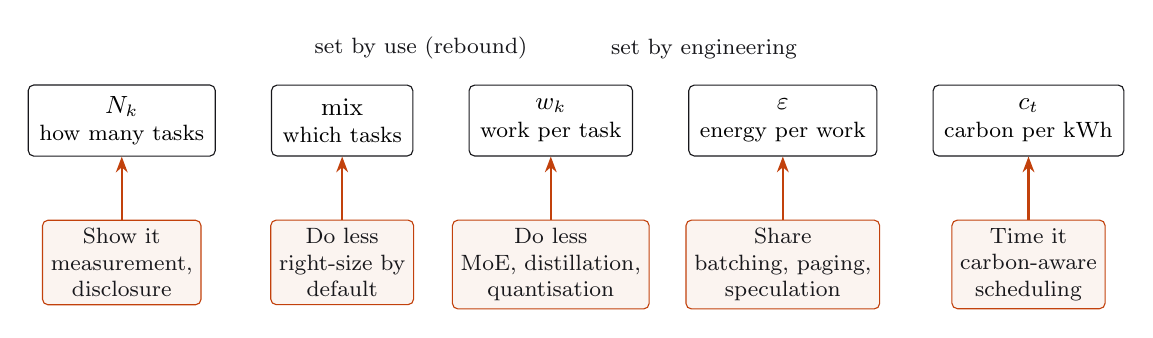
\begin{tikzpicture}[
  node distance=4mm and 6mm,
  box/.style={draw=ink, rounded corners=2pt, align=center, font=\small, inner sep=4pt, minimum height=9mm},
  lever/.style={draw=accent, text=ink, rounded corners=2pt, align=center, font=\footnotesize, inner sep=3pt, fill=accent!6},
  arr/.style={-{Stealth[length=2mm]}, accent, thick}]
  \node[box] (N) {$N_k$\\[-1pt]\footnotesize how many tasks};
  \node[box, right=7mm of N] (mix) {mix\\[-1pt]\footnotesize which tasks};
  \node[box, right=7mm of mix] (w) {$w_k$\\[-1pt]\footnotesize work per task};
  \node[box, right=7mm of w] (eps) {$\varepsilon$\\[-1pt]\footnotesize energy per work};
  \node[box, right=7mm of eps] (c) {$c_t$\\[-1pt]\footnotesize carbon per kWh};
  \node[lever, below=8mm of N] (show) {Show it\\measurement,\\disclosure};
  \node[lever, below=8mm of mix] (def) {Do less\\right-size by\\default};
  \node[lever, below=8mm of w] (less) {Do less\\MoE, distillation,\\quantisation};
  \node[lever, below=8mm of eps] (share) {Share\\batching, paging,\\speculation};
  \node[lever, below=8mm of c] (time) {Time it\\carbon-aware\\scheduling};
  \draw[arr] (show) -- (N); \draw[arr] (def) -- (mix); \draw[arr] (less) -- (w);
  \draw[arr] (share) -- (eps); \draw[arr] (time) -- (c);
  \node[font=\footnotesize, text=ink, above=2mm of mix, xshift=10mm] {set by use (rebound)};
  \node[font=\footnotesize, text=ink, above=2mm of eps, xshift=-10mm] {set by engineering};
\end{tikzpicture}
\caption{The identity $E=\sum_k N_k w_k \varepsilon$, $C=\sum_t E_t c_t$, with the intervention that acts on each factor. Engineering acts on the right-hand factors; the rebound effect lives in the left-hand ones.}
\label{fig:identity}
\end{figure}

% =====================================================================
\section{The Trap: Evidence of Rebound}\label{sec:trap}

\paragraph{Efficiency is real and large.} Google's study is the strongest evidence because it is a production measurement (grade~A) with a stated boundary: active accelerators, host CPU and memory, idle provisioned capacity, and data-centre overhead, with a fleet power usage effectiveness of $1.09$ \citep{elsworth2025}. Over May 2024 to May 2025 the median Gemini Apps text prompt's energy fell $33\times$ and its total carbon footprint $44\times$. The paper attributes the energy reduction to two multiplicative contributions: about $23\times$ from model improvements and about $1.4\times$ from better machine utilisation ($23 \times 1.4 \approx 32$). In the language of \eqref{eq:identity}, the first is mostly a reduction in $w$ and the second a reduction in $\varepsilon$; the extra carbon reduction beyond $33\times$ comes from cleaner electricity, a reduction in $c$. Across the industry, the IEA reports energy per task falling by at least $10\times$ per year \citep{iea2026}.

\paragraph{Demand rose anyway.} In 2025 global data-centre electricity rose $17\%$ and AI-focused data-centre electricity rose $50\%$ \citep{iea2026}. Electricity for AI-focused data centres is projected to roughly triple by 2030 \citep{iea2026}.

\paragraph{What the numbers imply.} Apply \eqref{eq:growth} to AI-focused data centres in 2025, taking the IEA's ``at least $10\times$'' as the per-task reduction ($e_k$ multiplied by at most $0.1$) and $1.5\times$ as the growth in total electricity. For both to hold, task-weighted demand $\sum_k N_k \cdot(\text{relative weight of }k)$ must have grown by a factor of at least
\[
  \frac{1.5}{0.1} = 15 .
\]
This is an illustrative bound, not a measurement. The per-task figure describes tasks of fixed capability, and some new capacity was built ahead of use, so the true demand multiplier is uncertain. But the order of magnitude is robust: demand for AI work must have grown roughly tenfold or more in a year, enough to overwhelm the efficiency gains.

\paragraph{Two channels of rebound.} The IEA identifies both. More tasks ($g_N>0$): adoption is growing quickly. Heavier tasks ($g_{\text{mix}}>0$): video generation, reasoning and agentic applications ``can consume hundreds or thousands of times more energy per query'' than simple text generation \citep{iea2026}. The pattern matches the economist William Jevons' 1865 observation that more efficient steam engines increased Britain's total coal use by making coal useful for more things \citep{jevons1865}. \citet{luccioni2025jevons} argue that such rebound effects undermine the assumption that technical efficiency alone will reduce AI's net environmental impact. The answer to RQ1 is therefore: \emph{per-task efficiency has been more than offset by growth in the number and weight of tasks.}

% =====================================================================
\section{Interventions: Four Moves}\label{sec:moves}

Table~\ref{tab:levers} organises interventions by the factor they change. We group them into four moves: \emph{do less} (reduce $w_k$, or shift the mix toward lighter tasks), \emph{share} (reduce $\varepsilon$ through utilisation), \emph{time it} (reduce $c_t$), and \emph{show it} (measure, which conditions all the others).

\begin{table}[h]
\centering
\small
\caption{Interventions, the factor each changes, and the strongest available evidence.}
\label{tab:levers}
\begin{tabularx}{\textwidth}{@{}p{2.6cm}cXXc@{}}
\toprule
Intervention & Factor & Reported effect & Caveat & Grade \\
\midrule
Right-sized / task-specific model & $w$, mix & General-purpose generative models are orders of magnitude more expensive than task-specific ones for the same task \citep{luccioni2024power}; $\sim\!40\times$ parameters gave $\sim\!40\times$ energy \citep{iea2025} & Capability may differ & B \\
Mixture of experts & $w$ & DeepSeek-R1 activates $\approx 5\%$ of parameters per token; a $2.5\times$ larger MoE model used only $\approx 45\%$ more energy \citep{iea2025} & All experts held in memory & B \\
Quantisation (8-bit) & $w$, $\varepsilon$ & Halves inference memory with no measured degradation up to 175B parameters \citep{dettmers2022} & Lower bit-widths need validation & B \\
Speculative decoding & $\varepsilon$ & $2$--$3\times$ faster decoding with identical outputs \citep{leviathan2023}; used in production to serve more responses per accelerator \citep{elsworth2025} & Needs a good draft model & B/A \\
Batching and paged KV-cache & $\varepsilon$ & Batching roughly halves energy per task \citep{iea2025}; PagedAttention raises throughput $2$--$4\times$ at equal latency \citep{kwon2023} & Latency; memory bound & B \\
Hardware generation & $\varepsilon$ & B200 $60\%$ more FLOP/W than H100, itself $80\%$ more than A100 \citep{iea2025} & Embodied energy & B \\
Temporal / spatial shifting & $c$ & Choosing a cleaner region can cut training carbon by over $70\%$ \citep{dodge2022}; deployed fleet-wide at Google \citep{radovanovic2023}; $\approx 50$\,GW of flexible capacity possible by 2035 \citep{iea2025} & Only deferrable work & A/B/D \\
Measurement and disclosure & all & Production methodology published \citep{elsworth2025}; EU AI Act requires documented energy use for general-purpose models \citep{euaiact} & Inference coverage weak & -- \\
\bottomrule
\end{tabularx}
\end{table}

\citet{patterson2022} reached a similar decomposition for training with their ``4Ms'' (model, machine, mechanisation, map), estimating that together they can reduce training energy by up to $100\times$ and emissions by up to $1000\times$. Our framework extends this to inference, which now dominates, and adds the demand-side factors $N_k$ and mix, which the 4Ms leave out and where the rebound occurs.

\paragraph{Do less.} The cheapest computation is the one not performed. The largest single choice is which model answers a request: routing simple requests to small or distilled models and reserving large reasoning models for problems that need them reduces both $w$ and the task mix. Sparse architectures (mixture of experts) reduce active work per token, and quantisation reduces the bytes moved per operation. Inference at small batch sizes is limited by memory bandwidth rather than arithmetic \citep{leviathan2023}, so fewer bytes is close to less energy.

\paragraph{Share.} Each decoding step must stream the model's weights from memory regardless of how many requests it serves. Sharing that fixed cost across requests (batching) is the main utilisation lever; \S\ref{sec:batch} analyses it.

\paragraph{Time it.} The same computation emits different amounts of CO$_2$ depending on when and where it runs; in California carbon intensity ranges from under $70$\,g/kWh in the afternoon to over $300$ at night \citep{mittr2025}. Deferrable work (training, batch inference, video processing) can be moved; \S\ref{sec:sched} gives an optimal algorithm.

\paragraph{Show it.} In early 2025 no major AI company disclosed per-prompt energy use \citep{mittr2025}. Without measurement, efficiency gains cannot be distinguished from rebound and policy cannot target the left-hand side of \eqref{eq:growth}. This answers RQ3 in part: measurement is the condition under which the other moves can be verified.

% =====================================================================
\section{Algorithmic Analysis}\label{sec:algorithms}

\subsection{Batching as amortisation}\label{sec:batch}
Let $F$ be the fixed cost of one decoding step (dominated by reading the weights), $v$ the marginal cost per request in the batch, and $b$ the batch size. The cost per request is
\begin{equation}
  \text{cost}(b) = \frac{F}{b} + v .
\end{equation}
This is amortised analysis in the sense of \citet{clrs}: an expensive operation spread over many cheap ones, as in a dynamic array whose occasional doubling costs $O(1)$ per insertion on average. The model predicts the IEA's two observations: batching roughly halves energy per task, and gains diminish with $b$, since doubling $b$ saves only $F/(2b)$ \citep{iea2025}. It also predicts the constraint: each request stores a key--value cache of size $m$, so with memory $M$ and weights $W$, $b \le \lfloor (M-W)/m \rfloor$. \citet{kwon2023} found that conventional serving systems used only $20.4$--$38.2\%$ of KV-cache memory for actual token states, the rest being lost to fragmentation and over-reservation. PagedAttention allocates the cache in fixed-size pages, as an operating system allocates virtual memory, which effectively reduces the wasted memory per request and so raises the feasible $b$. That is the mechanism behind its $2$--$4\times$ throughput gain.

\subsection{Speculative decoding as a geometric series}\label{sec:spec}
Autoregressive decoding produces one token per call to the large model. Speculative decoding \citep{leviathan2023} lets a small draft model propose $\gamma$ tokens, which the large model verifies in a single parallel call; a modified rejection-sampling rule guarantees that the output distribution is exactly that of the large model. If each drafted token is accepted independently with probability $\alpha$, the number of tokens produced per large-model call is $1$ plus the length of the accepted prefix, whose expectation is a truncated geometric series:
\begin{equation}
  \mathbb{E}[\text{tokens per call}] \;=\; \sum_{i=0}^{\gamma} \alpha^{i} \;=\; \frac{1-\alpha^{\gamma+1}}{1-\alpha}.
\end{equation}
With $\alpha=0.8$ and $\gamma=4$ this is $\approx 3.4$ tokens per call instead of one. Because the large model is memory-bound, verifying several tokens costs about as much as generating one, so fewer large-model calls means fewer passes over the weights. The reported $2$--$3\times$ speed-ups are consistent with this analysis once the draft model's own cost is included. The idea is speculative execution, familiar from branch prediction, and it rests on an asymmetry that also motivates the class NP: checking a proposed answer can be much cheaper than finding one. (Here the asymmetry comes from parallel verification, not from complexity classes; the analogy is intuitive only.) The price is wasted work on rejected drafts.

\subsection{Carbon-aware scheduling}\label{sec:sched}
A deferrable job needs energy $E$ before a deadline. Divide the window into $n$ slots (hours) with carbon intensities $c_1,\dots,c_n$ and a power cap allowing at most $P$ energy per slot. Choose $x_t$, the energy drawn in slot $t$:
\begin{equation}
  \min_{x} \sum_{t=1}^{n} c_t\,x_t
  \quad\text{s.t.}\quad \sum_{t=1}^{n} x_t = E,\qquad 0 \le x_t \le P,
  \label{eq:sched}
\end{equation}
assuming feasibility, $E \le nP$. The continuous-time version, $\min \int_0^T C(t)P(t)\,dt$ subject to $\int_0^T P(t)\,dt = E$ and $0\le P(t)\le P_{\max}$, has the same structure, and its optimum is a threshold policy: run at full power whenever $C(t)$ is below a level $\tau$ and not at all above it.

\begin{algorithm}[h]
\caption{Greedy carbon-aware schedule}
\label{alg:greedy}
\begin{algorithmic}[1]
\Require intensities $c_1,\dots,c_n$; cap $P$; energy $E \le nP$
\State order slots so that $c_{\pi(1)} \le c_{\pi(2)} \le \dots \le c_{\pi(n)}$
\State $R \gets E$; \quad $x_t \gets 0$ for all $t$
\For{$k = 1, 2, \dots$ \textbf{while} $R > 0$}
  \State $x_{\pi(k)} \gets \min(P, R)$; \quad $R \gets R - x_{\pi(k)}$
\EndFor
\State \Return $x$
\end{algorithmic}
\end{algorithm}

\begin{proposition}\label{prop:greedy}
Algorithm~\ref{alg:greedy} returns an optimal solution of \eqref{eq:sched}.
\end{proposition}
\begin{proof}
Let $x$ be optimal and suppose slots $i,j$ satisfy $c_i < c_j$, $x_i < P$ and $x_j > 0$. Set $\delta = \min(P-x_i,\,x_j) > 0$ and move $\delta$ energy from $j$ to $i$. Feasibility is preserved and the objective changes by $\delta(c_i-c_j)<0$, contradicting optimality. Hence in any optimal solution no slot receives energy while a strictly cleaner slot has spare capacity. Slots of equal intensity can exchange energy at zero cost. The greedy solution satisfies the same property, and any two solutions with this property have equal cost, so the greedy solution is optimal.
\end{proof}

\begin{proposition}
Problem \eqref{eq:sched} can be solved in $O(n)$ time.
\end{proposition}
\begin{proof}
Let $q=\lfloor E/P\rfloor$ and $r = E - qP$; if $q=n$, every slot is full and we are done. By Proposition~\ref{prop:greedy} an optimal solution fills the $q$ cleanest slots completely and gives $r$ to the $(q{+}1)$-th cleanest. Linear-time selection \citep{clrs} finds the $(q{+}1)$-th smallest intensity $c^*$ in $O(n)$. One pass then assigns $P$ to slots with $c_t<c^*$, and the remaining energy to slots with $c_t=c^*$ (breaking ties arbitrarily), also in $O(n)$.
\end{proof}

\begin{remark}
The problem is a fractional knapsack in disguise: linear costs and divisible energy make greedy optimal. With indivisible jobs, start-up costs, multiple jobs sharing capacity, or per-job deadlines, it becomes a min-cost flow or integer programme. Real systems also act on \emph{forecasts} of $c_t$; Google's system plans next-day capacity curves with risk-aware optimisation rather than a single greedy pass \citep{radovanovic2023}. With MIT's California figures, moving a four-hour job from night ($\approx 300$\,g/kWh) to afternoon ($\approx 70$\,g/kWh) cuts its emissions by about $(300-70)/300 \approx 77\%$; this is illustrative, and real savings depend on the day's curve and the job's slack.
\end{remark}



\subsection{Budgeted model routing as multiple-choice knapsack}\label{sec:router}
``Do less'' becomes an optimisation problem when a provider must serve a batch of $n$ requests under an energy budget $B$. Request $i$ may be served by model $j\in\{1,\dots,m\}$ at energy $w_{ij}$ with quality $q_{ij}$. Choosing exactly one model per request to maximise $\sum_i q_{i,j(i)}$ subject to $\sum_i w_{i,j(i)}\le B$ is the \emph{multiple-choice knapsack problem}, NP-hard in general but solvable in pseudo-polynomial time. With energies rounded up to integer units,
\begin{equation}
  \mathrm{best}_i(b) \;=\; \max_{j:\,w_{ij}\le b}\;\bigl[\mathrm{best}_{i-1}(b-w_{ij}) + q_{ij}\bigr],
  \qquad \mathrm{best}_0(0)=0,
\end{equation}
computed in $O(nmB)$ time. Rounding up guarantees the real energy never exceeds the budget. Greedy by quality per watt-hour is optimal only for the fractional relaxation, since a request cannot be served by a fraction of a model, so dynamic programming is required.


\subsection{Capping the total: an anti-rebound policy}\label{sec:cap}
Existing tools each address one factor of \eqref{eq:identity} for a single job: when to run (the Green Software Foundation's Carbon Aware SDK), which model to call (RouteLLM), how to batch (vLLM) and how to measure (CodeCarbon). By the argument of \S\ref{sec:trap}, making each job cheaper is precisely what feeds the rebound. We therefore add a policy that fixes the \emph{total}: for each period, energy is capped at a budget $B$ and a multiple-choice knapsack (\S\ref{sec:router}) chooses, for every request, a model or the option to defer it (zero energy, zero quality), maximising total quality subject to $\sum w \le B$.

\paragraph{Is a cap not just a rate limit?} Providers already cap usage. In March 2025, demand for ChatGPT's new image generator led OpenAI's chief executive to report that the company's GPUs were ``melting'' and to impose temporary rate limits, including three images a day for free users, while the system was made more efficient \citep{altman2025}. Such limits are explicitly temporary: they hold demand back until efficiency catches up, after which demand grows into the new headroom, which is the rebound cycle again. A rate limit also serves requests first come, first served, blind to what each request needs. We therefore compare it directly with the knapsack under the \emph{same} energy.

We simulated one year monthly on a seeded sample of 120 requests (illustrative difficulty mix; IEA laboratory energies per answer), with per-task energy falling $10\times$ per year and task-weighted demand growing $15\times$ per year, the rates implied by the IEA's 2025 figures (\S\ref{sec:trap}). Policy~A sends each request to the cheapest adequate model, a per-job efficiency policy like today's tools, with no cap. Policy~R is a rate limit: the same cap as~B, but requests are served in arrival order on their ideal model until the energy runs out, and the rest are refused. Policy~B applies the cap at month-0 energy and lets the knapsack choose. Table~\ref{tab:cap} reports month~12.

\begin{table}[h]
\centering\small
\caption{One-year simulation at month 12 (\texttt{effitrap experiment}). Energy relative to month 0.}
\label{tab:cap}
\begin{tabular}{@{}rcccc@{}}
\toprule
Demand growth / yr & A: energy (no cap) & B: energy (cap) & R: answered & B: answered / full quality \\
\midrule
$15\times$ & $1.5\times$ & $0.89\times$ & 61\% & 100\% / 95\% \\
$30\times$ & $3.0\times$ & $0.94\times$ & 38\% & 100\% / 91\% \\
$60\times$ & $6.0\times$ & $0.95\times$ & 29\% & 72\% / 72\% \\
$120\times$ & $12.0\times$ & $0.97\times$ & 25\% & 37\% / 37\% \\
\bottomrule
\end{tabular}
\end{table}

At the IEA-implied pace the cap holds total energy flat while answering every request, by moving about 5\% of the hardest requests to the next-smaller model. With identical energy the rate limit answers only 61\%: it refuses people, whereas the knapsack right-sizes them. In every month and at every growth rate tested, the knapsack answered at least as many requests as the rate limit (a property checked in the test suite). When demand outruns efficiency by more, the cap still holds but must defer work, which makes the trade-off explicit rather than hiding it in a growing electricity bill. The results depend on the illustrative difficulty mix and quality scores and should be read as a demonstration of mechanism, not a forecast. Nor does the cap defeat the rebound: if demand grows $60\times$ a year, even the knapsack must defer 28\% of requests. In keeping with the No Free Lunch theorem, an algorithm can spend a budget well; it cannot decide what the budget should be. That choice belongs to people, firms and regulators.

% =====================================================================
\section{Implementation and Evaluation}\label{sec:impl}

We implemented every algorithm in this paper as an open-source Python package, \texttt{effitrap} (core library with no dependencies; command-line tool; optional HTTP API built on FastAPI; Docker image; continuous integration on Python 3.9--3.12). Table~\ref{tab:modules} maps modules to moves. A \texttt{run} command turns the scheduler into a practical tool: given a job length, a deadline window and either a carbon-intensity file or Great Britain's public half-hourly forecast, it computes the cleanest contiguous window (jobs that cannot checkpoint cannot pause), sleeps until then and launches the user's command. A companion browser playground implements all four moves interactively for non-programmers.

\paragraph{A model-agnostic gate.} The future of AI deployment is multi-model: providers already sell families of small, fast models and large, slow ones. Something must decide which model answers each request, and when. \texttt{effitrap} does this without touching any model. Its \texttt{Gate} class sits between an application and any AI service; one call before each request returns a model name (or ``wait'') and charges an energy ledger, after which the application makes its usual API call:
\begin{center}\small
\texttt{choice = gate.pick(prompt);\ \ client.messages.create(model=choice.model, ...)}
\end{center}
For a single request, \texttt{pick} chooses the smallest model whose quality meets the request's estimated difficulty, falling back to the best affordable model, or to waiting, when the budget is tight. For a group of requests, \texttt{pick\_many} solves the multiple-choice knapsack of \S\ref{sec:router} exactly. Difficulty is estimated by a deliberately simple length-and-keyword rule that a trained router such as RouteLLM can replace. A developer who uses only one provider still benefits: Claude, for instance, is offered as Haiku, Sonnet and Opus, which \texttt{effitrap} ships as a preset, and requests that can wait are held for the cleanest hour and sent as a single Message Batch, which Anthropic bills at 50\% of standard prices \citep{anthropicbatch}. Energy per answer for commercial models is not published, so the preset uses IEA-based stand-ins that users can replace with measurements.

\paragraph{Forecasts.} The \texttt{run} command plans against a carbon-intensity forecast: Great Britain's free half-hourly national forecast \citep{carbonintensity}, any zone covered by Electricity Maps (with a token that includes forecast access) \citep{electricitymaps}, or a user-supplied file. A real forecast recorded on 24 November 2026 (97 half-hour values) is stored with the tests; on it, the cleanest four-hour window in the next 24 hours starts at 01:00 rather than 16:00 and emits 56\% less carbon. Three safeguards address the obvious objections. While waiting, the command re-fetches a live forecast every 30 minutes and moves the start if a cleaner window appears; if a download fails it keeps the last plan, and if no plan exists it starts at once; and in every case the deadline is never missed. To test sensitivity to forecast error, we perturbed every hour of 300 synthetic days by up to $\pm30\%$, planned on the perturbed values and scored the plan on the true ones: waiting still cut emissions by 54\% on average, was worse than starting immediately on 8 days, and was at worst 22\% worse.

\begin{table}[h]
\centering\small
\caption{\texttt{effitrap} modules.}
\label{tab:modules}
\begin{tabularx}{\textwidth}{@{}llXc@{}}
\toprule
Move & Module & Algorithm & Complexity \\
\midrule
Do less & \texttt{router} & multiple-choice knapsack DP (\S\ref{sec:router}) & $O(nmB)$ \\
Share & \texttt{batching} & amortised cost; largest feasible batch by binary search (\S\ref{sec:batch}) & $O(\log b)$ \\
Share & \texttt{speculative} & closed form, Monte Carlo check, best draft length (\S\ref{sec:spec}) & $O(\gamma)$ \\
Time it & \texttt{schedule} & greedy, quickselect; run-now and flexible-start baselines (\S\ref{sec:sched}) & $O(n)$ expected \\
Show it & \texttt{identity}, \texttt{units} & identity \eqref{eq:identity}, rebound bound, everyday units & $O(k)$ \\
Cap it & \texttt{budget}, \texttt{gate} & energy ledger; knapsack with a ``defer'' option; one-line gate (\S\ref{sec:cap}) & $O(nmB)$ \\
Time it & \texttt{carbon} & GB and Electricity Maps forecasts; re-planning; sliding window & $O(n)$ \\
Evaluate & \texttt{experiment} & one-year simulation: no cap, rate limit, knapsack (\S\ref{sec:cap}) & -- \\
\bottomrule
\end{tabularx}
\end{table}

\paragraph{Correctness.} Every test solves a problem two ways and compares: a fast algorithm against a slow, trusted oracle, on seeded random inputs that anyone can replay. The suite (49 checks run on 906 random cases) verifies: greedy and quickselect schedules agree on 300 random instances including ties; both match a linear-programming oracle (SciPy/HiGHS) on 100 instances; the exchange invariant of Proposition~\ref{prop:greedy} holds directly; neither baseline ever beats the optimum; the knapsack router equals exhaustive search on 120 random instances and never exceeds its budget; binary-searched batch sizes equal a linear scan; the speculative-decoding closed form matches 200{,}000-trial simulations within $1\%$; with equal energy the knapsack never answers fewer requests than a rate limit; the budget never exceeds its cap; the forecast parsers read the real recorded response and the documented Electricity Maps format; re-planning moves the start when a forecast changes, survives download failures and never misses a deadline (50 randomised runs); the forecast-error results above hold; and the Claude example routes easy and hard prompts to different models and batches deferrable ones, run against a fake client. Two further tests encode the worked examples used in the talk: greedy selection by value per watt-hour scores 7 where the optimum is 10 on a three-job instance (so greedy is not optimal for indivisible jobs), and the dynamic programme reproduces the hand-worked three-question table exactly. The suite exposed one genuine defect during development: when a job required every slot, the quickselect implementation assigned the partial slot to the wrong hour. The fix routes that case through the same threshold logic as all others.

\paragraph{Performance.} Table~\ref{tab:bench} reports median wall time on random instances (CPython, single core).\footnote{Measured in the build environment; absolute times vary by machine.} At small $n$ sorting's low constant factor wins; at $10^6$ slots expected-linear selection is about $1.6\times$ faster, as the asymptotics predict. The knapsack router solves 200 requests with a 400\,Wh budget at $0.1$\,Wh resolution in about a quarter of a second, consistent with its $O(nmB)$ bound.

\begin{table}[h]
\centering\small
\caption{Scheduler running time (median of 3 runs).}
\label{tab:bench}
\begin{tabular}{@{}rrr@{}}
\toprule
$n$ slots & greedy (sort) & quickselect \\
\midrule
$10^3$ & 0.1 ms & 0.3 ms \\
$10^4$ & 1.6 ms & 1.2 ms \\
$10^5$ & 26.9 ms & 19.3 ms \\
$10^6$ & 270 ms & 172 ms \\
\bottomrule
\end{tabular}
\end{table}

\paragraph{Effect.} On an illustrative 24-hour carbon curve shaped like MIT's California description (not measured data), a four-hour job emits $1{,}185$ units if run immediately and $269$ under the optimal schedule, a $77\%$ reduction; here the best contiguous window (flexible start) happens to equal the optimum because the clean hours are adjacent. With illustrative batching constants, reducing KV-cache waste from $70\%$ to $4\%$ raises the feasible batch from 20 to 64 and lowers modelled energy per request from 10 to 6.7\,J. For speculative decoding with $\alpha=0.8$ and a draft $20\times$ cheaper than the target, the optimal draft length is $\gamma=8$, giving $4.33$ expected tokens per target call (simulation: $4.31$) and an expected speed-up of about $3.1\times$. Pricing MIT's ``day of AI use'' (15 texts, 10 images, 3 videos) with the IEA's laboratory figures gives $366.5$\,Wh, about $0.37$\,kWh or six laptop charges, of which $94\%$ is video.

% =====================================================================
\section{Discussion and Recommendations}\label{sec:policy}

Three conclusions follow from the identity and the evidence.

\emph{First, engineering is working.} The $33\times$ result is a production measurement, and its decomposition ($\approx 23\times$ model, $\approx 1.4\times$ utilisation, plus cleaner power) shows that the ``do less'', ``share'' and ``time it'' moves deliver in practice \citep{elsworth2025}.

\emph{Second, engineering alone is insufficient.} Equation~\eqref{eq:growth} shows that falling $w$ and $\varepsilon$ cannot guarantee falling $E$ while $N$ and the task mix grow faster, and the 2025 data indicate they did \citep{iea2026}. Lower costs may even accelerate demand, as the IEA noted when DeepSeek's efficiency gains raised the same question \citep{iea2025}.

\emph{Third, timing reduces emissions independently of volume.} Carbon-aware scheduling acts on $c_t$, which rebound does not touch, and the IEA estimates that brief flexibility could let much more data-centre load fit on existing grids \citep{iea2025}.

We therefore recommend:
\begin{enumerate}[leftmargin=*,itemsep=2pt]
  \item \textbf{Measure inference in production and publish it.} Adopt a common boundary such as Google's comprehensive methodology \citep{elsworth2025}, and extend regulatory documentation, which in the EU AI Act centres on model development, to cover inference \citep{euaiact}.
  \item \textbf{Make the lightest adequate model the default.} Route requests by difficulty, so that reasoning and video, which can cost hundreds to thousands of times more \citep{iea2026}, are used when they add value, not by default.
  \item \textbf{Make deferrable work carbon-aware by default.} Training and batch jobs should carry deadlines and be scheduled against forecast carbon intensity (\S\ref{sec:sched}).
  \item \textbf{Report totals alongside efficiency.} Efficiency claims should be accompanied by absolute energy and emissions, so that rebound is visible rather than hidden behind per-task improvements \citep{luccioni2025jevons}.
\end{enumerate}

\paragraph{The other direction.} AI can also reduce energy use elsewhere. The IEA estimates that existing applications could unlock up to 175\,GW of transmission capacity on existing lines and cut energy-related emissions by around $5\%$ by 2035, while cautioning that this is no substitute for policy \citep{iea2025}.

% =====================================================================
\section{Limitations}\label{sec:limits}
\begin{itemize}[leftmargin=*,itemsep=1pt]
  \item The strongest efficiency evidence comes from one firm's internal telemetry, which outsiders cannot verify; it covers text prompts, not images, video or agents \citep{elsworth2025}.
  \item Laboratory figures (grade B) usually count accelerator energy only and use open models, which may differ from commercial systems.
  \item The implied-demand bound in \S\ref{sec:trap} combines an industry-wide per-task trend with an aggregate electricity figure; it indicates an order of magnitude, not a precise value.
  \item The algorithmic models are deliberately simple. They explain observed effects (diminishing returns to batching, speculative speed-ups, the value of slack) rather than predict exact savings.
  \item The tool plans with estimates and does not measure electricity; energy per answer for commercial models is unpublished, so its defaults are IEA-based stand-ins. Difficulty is estimated by a simple rule, and single-request \texttt{pick} is myopic (early requests can use up a budget); grouping requests and using \texttt{pick\_many} avoids this.
  \item Live forecasts are free only for Great Britain; elsewhere they need a paid data service or the user's own data. The forecast-error test uses synthetic days.
  \item Projections (grade D) are scenarios whose range is wide; the IEA's 2035 cases span roughly $700$ to $1{,}700\TWh$ \citep{iea2025}.
\end{itemize}

% =====================================================================
\section{Conclusion}
Turing's machine can solve anything solvable; it was never going to be free. AI is caught in an efficiency trap: energy per task is falling faster than in almost any energy technology on record, yet total electricity demand is rising, because the number and weight of tasks are growing faster still. The factor identity $E=\sum_k N_k w_k \varepsilon$, $C=\sum_t E_t c_t$ shows where each intervention acts and why engineering on $w$ and $\varepsilon$ cannot by itself control $E$. Four interventions have clean algorithmic cores (routing, a geometric series, amortisation, and a provably optimal greedy schedule), each with a price. A fifth acts on the total: an energy budget spent by a knapsack, which with the same energy answers far more people than the rate limits providers use today. All are implemented in \texttt{effitrap}, a model-agnostic door between applications and any AI, tested against independent oracles. None of this abolishes the trade-off. An algorithm can spend a budget wisely; choosing the budget, and measuring honestly enough to see whether savings are kept, remains a human decision.

% =====================================================================
\begin{thebibliography}{99}\small

\bibitem[Altman(2025)]{altman2025}
S.~Altman.
\newblock Post on X, 27 March 2025, on ChatGPT image-generation demand and temporary rate limits.
\newblock Reported in \emph{Fortune}, ``Sam Altman says ChatGPT's viral image-generation AI is `melting' OpenAI's GPUs'', 28 March 2025.

\bibitem[Anthropic(2026)]{anthropicbatch}
Anthropic.
\newblock Batch processing (Message Batches API).
\newblock Claude Platform documentation, accessed November 2026.

\bibitem[Carbon Intensity API(2026)]{carbonintensity}
National Energy System Operator (Great Britain).
\newblock Carbon Intensity API, national forecast endpoint \texttt{/intensity/\{from\}/fw48h}.
\newblock api.carbonintensity.org.uk, accessed 24 November 2026.

\bibitem[Cormen et al.(2022)]{clrs}
T.~H. Cormen, C.~E. Leiserson, R.~L. Rivest, and C.~Stein.
\newblock \emph{Introduction to Algorithms}, 4th ed.
\newblock MIT Press, 2022.

\bibitem[Dettmers et al.(2022)]{dettmers2022}
T.~Dettmers, M.~Lewis, Y.~Belkada, and L.~Zettlemoyer.
\newblock LLM.int8(): 8-bit matrix multiplication for transformers at scale.
\newblock In \emph{Advances in Neural Information Processing Systems (NeurIPS)}, 2022. arXiv:2208.07339.

\bibitem[Dodge et al.(2022)]{dodge2022}
J.~Dodge, T.~Prewitt, R.~Tachet des Combes, E.~Odmark, R.~Schwartz, E.~Strubell, A.~S. Luccioni, N.~A. Smith, et~al.
\newblock Measuring the carbon intensity of AI in cloud instances.
\newblock In \emph{ACM Conference on Fairness, Accountability, and Transparency (FAccT)}, pp.~1877--1894, 2022.

\bibitem[Elsworth et al.(2025)]{elsworth2025}
C.~Elsworth et~al.
\newblock Measuring the environmental impact of delivering AI at Google scale.
\newblock arXiv:2508.15734, 2025.

\bibitem[Electricity Maps(2026)]{electricitymaps}
Electricity Maps.
\newblock API reference: \texttt{/v3/carbon-intensity/forecast}.
\newblock Accessed November 2026.

\bibitem[European Union(2024)]{euaiact}
European Union.
\newblock Regulation (EU) 2024/1689 (Artificial Intelligence Act), Article 53 and Annex XI.
\newblock \emph{Official Journal of the European Union}, 2024.

\bibitem[IEA(2025)]{iea2025}
International Energy Agency.
\newblock \emph{Energy and AI}.
\newblock IEA, Paris, 2025. CC BY 4.0.

\bibitem[IEA(2026)]{iea2026}
International Energy Agency.
\newblock \emph{Key Questions on Energy and AI}.
\newblock IEA, Paris, April 2026.

\bibitem[Jevons(1865)]{jevons1865}
W.~S. Jevons.
\newblock \emph{The Coal Question}.
\newblock Macmillan, London, 1865.

\bibitem[Kaplan et al.(2020)]{kaplan2020}
J.~Kaplan, S.~McCandlish, T.~Henighan, et~al.
\newblock Scaling laws for neural language models.
\newblock arXiv:2001.08361, 2020.

\bibitem[Kwon et al.(2023)]{kwon2023}
W.~Kwon, Z.~Li, S.~Zhuang, Y.~Sheng, L.~Zheng, C.~H. Yu, J.~E. Gonzalez, H.~Zhang, and I.~Stoica.
\newblock Efficient memory management for large language model serving with PagedAttention.
\newblock In \emph{ACM Symposium on Operating Systems Principles (SOSP)}, 2023.

\bibitem[Leviathan et al.(2023)]{leviathan2023}
Y.~Leviathan, M.~Kalman, and Y.~Matias.
\newblock Fast inference from transformers via speculative decoding.
\newblock In \emph{International Conference on Machine Learning (ICML)}, PMLR 202:19274--19286, 2023.

\bibitem[Luccioni et al.(2024)]{luccioni2024power}
A.~S. Luccioni, Y.~Jernite, and E.~Strubell.
\newblock Power hungry processing: Watts driving the cost of AI deployment?
\newblock In \emph{ACM FAccT}, 2024.

\bibitem[Luccioni et al.(2025)]{luccioni2025jevons}
A.~S. Luccioni, E.~Strubell, and K.~Crawford.
\newblock From efficiency gains to rebound effects: The problem of Jevons' paradox in AI's polarized environmental debate.
\newblock In \emph{ACM FAccT}, 2025.

\bibitem[O'Donnell and Crownhart(2025)]{mittr2025}
J.~O'Donnell and C.~Crownhart.
\newblock We did the math on AI's energy footprint. Here's the story you haven't heard.
\newblock \emph{MIT Technology Review}, 20 May 2025.

\bibitem[Our World in Data(2026)]{owid2026}
Our World in Data.
\newblock How much energy do data centers and artificial intelligence use?
\newblock July 2026.

\bibitem[Patterson et al.(2022)]{patterson2022}
D.~Patterson, J.~Gonzalez, U.~H\"olzle, Q.~Le, C.~Liang, L.-M. Munguia, D.~Rothchild, D.~So, M.~Texier, and J.~Dean.
\newblock The carbon footprint of machine learning training will plateau, then shrink.
\newblock \emph{IEEE Computer}, 2022. arXiv:2204.05149.

\bibitem[Radovanovi\'c et al.(2023)]{radovanovic2023}
A.~Radovanovi\'c, R.~Koningstein, I.~Schneider, B.~Chen, A.~Duarte, B.~Roy, D.~Xiao, et~al.
\newblock Carbon-aware computing for datacenters.
\newblock \emph{IEEE Transactions on Power Systems}, 2023. arXiv:2106.11750.

\bibitem[Shehabi et al.(2024)]{shehabi2024}
A.~Shehabi, S.~J. Smith, A.~Hubbard, A.~Newkirk, N.~Lei, M.~A.~B. Siddik, B.~Holecek, J.~Koomey, E.~Masanet, and D.~Sartor.
\newblock \emph{2024 United States Data Center Energy Usage Report}.
\newblock Lawrence Berkeley National Laboratory, LBNL-2001637, 2024.

\bibitem[Turing(1936)]{turing1936}
A.~M. Turing.
\newblock On computable numbers, with an application to the Entscheidungsproblem.
\newblock \emph{Proceedings of the London Mathematical Society}, s2-42(1):230--265, 1936.

\bibitem[Wolpert and Macready(1997)]{wolpert1997}
D.~H. Wolpert and W.~G. Macready.
\newblock No free lunch theorems for optimization.
\newblock \emph{IEEE Transactions on Evolutionary Computation}, 1(1):67--82, 1997.

\end{thebibliography}

\end{document}
